\documentclass[conference]{IEEEtran}
\usepackage{cite}
\usepackage{amsmath,amssymb}
\usepackage{graphicx}
\usepackage{booktabs}
\usepackage{array}
\usepackage{url}
\usepackage{tikz}
\usetikzlibrary{arrows.meta,positioning}
\usepackage{balance}
\newcommand{\todo}[1]{\textbf{TODO: #1}}
\begin{document}
\title{Topology-Aware Adaptive Fusion of WiFi RSSI and Visible-Light Signals for Robust Simulated Indoor Positioning}
\author{\IEEEauthorblockN{Shahriar Rizvi, Tasfia Jannat Tasfi, and Dr. Md. Nazrul Islam Mondal}
\IEEEauthorblockA{Shahriar Rizvi and Tasfia Jannat Tasfi: Department of Computer Science and Engineering,\\
Rajshahi University of Engineering \& Technology, Rajshahi, Bangladesh\\
Dr. Md. Nazrul Islam Mondal: \todo{confirm full affiliation}\\
Emails: \todo{add verified author emails}}}
\maketitle

\begin{abstract}
This paper presents a simulation-based robustness study of hybrid indoor positioning from WiFi received-signal-strength-indicator (RSSI)-like measurements and visible-light-positioning (VLP) intensity-like measurements. The evaluated framework applies moving-average, median, and exponential-moving-average digital signal processing (DSP) filters; represents location evidence as probability maps; smooths spatial priors on a room graph; and selects among predefined fusion modes with a lightweight reliability-aware adaptive policy. Experiments use a $10\,\mathrm{m}\times10\,\mathrm{m}$ room, a $10\times10$ candidate-cell grid, three WiFi access points, four LED anchors, synthetic walking trajectories, and five repeated seeds under clean, WiFi-degraded, VLP-blocked, and mixed-dynamic scenarios. Adaptive fusion is not universally best: static fusion gives the lowest clean-case mean error, and VLP-only estimation is best when only WiFi is degraded. Under optical blockage and mixed degradation, however, adaptive fusion reduces mean error by approximately 25.51\% and 18.90\%, respectively, relative to static fusion. A small smartphone-based physical sanity check shows distance- and blockage-sensitive trends in RSSI and app-estimated light intensity. This check motivates the simulated degradations; it is not a full real-world localization validation.
\end{abstract}
\begin{IEEEkeywords}
indoor positioning, WiFi RSSI, visible-light positioning, sensor fusion, graph signal processing, DSP filtering
\end{IEEEkeywords}

\section{Introduction}
Reliable indoor positioning remains difficult when satellite signals are unavailable and inexpensive sensing modalities are individually fragile. WiFi RSSI is widely accessible, but multipath and environmental change disturb the observed signal. Visible-light positioning (VLP) provides a complementary optical cue, yet line-of-sight blockage and intensity variation can weaken its evidence. Classic WiFi systems established RF fingerprinting and probabilistic location estimation \cite{bahl2000radar,youssef2005horus}; later work continued to study robust wireless localization and practical WiFi positioning principles \cite{ayyalasomayajula2020dloc,dai2023wifi}. VLP surveys likewise identify optical blockage and implementation constraints as central practical issues \cite{do2016vlc,luo2017vlpstate,afzalan2019vlp}.

A fixed fusion rule is attractive because it is simple, but it can retain a damaged modality exactly when the other modality should dominate. This paper studies a physically motivated, reproducible alternative: a lightweight reliability-aware adaptive fusion policy using DSP-filtered signal streams and graph-smoothed probability priors. The policy is transparent and uses predefined modes; it is not end-to-end learning and is not presented as a new reinforcement-learning (RL) algorithm. Early planning considered RL-style adaptive fusion, motivated in part by prior RL-based fusion work \cite{salimibeni2022rlfusion}, but the final implementation deliberately favors traceability.

The contributions are threefold: (1) a reproducible stress test for complementary RSSI-like and VLP intensity-like evidence under controlled degradation; (2) a compact DSP--graph-signal-processing (GSP) pipeline with a reliability-aware mode-selection policy; and (3) a repeated-seed analysis showing where static, single-modality, and adaptive fusion each work best. The central claim is intentionally narrow: reliability-aware adaptive fusion improves robustness under simulated optical blockage and mixed degradation.

\section{Related Work}
WiFi positioning ranges from RSSI fingerprinting to learned wireless localization \cite{bahl2000radar,youssef2005horus,ayyalasomayajula2020dloc,dai2023wifi}. Our low-resource study does not use channel state information or a calibrated building fingerprint database. It instead tests how RSSI-like evidence behaves when noise bursts and shadowing are controlled in simulation.

VLP uses illumination infrastructure as location anchors. Surveys describe received-signal-strength, angle, imaging, and hybrid variants, along with line-of-sight and hardware constraints \cite{do2016vlc,luo2017vlpstate,afzalan2019vlp}. Recent tracking work illustrates practical optical estimation using extended Kalman filtering \cite{saengudomlert2025aeu_ekf_vlp}. Hybrid RF--optical and LiFi--WiFi studies further motivate complementary sensing \cite{lu2025rfvlp,mustafa2025lifiwifi}. We do not claim direct comparison to those systems because our evaluation is simulated.

GSP provides tools for processing signals defined on irregular domains \cite{shuman2013gsp,ortega2018gsp}. Indoor grids are natural graphs: adjacent cells encode local spatial continuity. Related graph-based fingerprint work uses graph structure for augmentation \cite{chen2023graphfingerprint}. Our narrower use is graph smoothing of cell-probability priors before reliability-aware fusion.

\section{System Model and Problem Setup}
\subsection{Room, anchors, and signal models}
The simulated room is divided into 100 candidate cells. Three WiFi access points and four LED anchors are placed as shown in Fig.~\ref{fig:layout}. A 100-step synthetic walking path is generated for each seed. For a candidate position $\mathbf{x}$ and access point $i$, the expected RSSI-like value is
\begin{equation}
 r_i(\mathbf{x})=P_0-10n\log_{10}\!\left(\max(d_i(\mathbf{x}),d_{\min})\right),
 \label{eq:wifi}
\end{equation}
where $P_0=-40$ dBm and $n=2.2$. Gaussian noise, shadowing, and multipath-like bursts are applied according to the scenario. For LED $j$, the expected intensity-like value is
\begin{equation}
 \ell_j(\mathbf{x})=\frac{P_{\mathrm{LED}} h^2}{\left(d_{j,h}^2(\mathbf{x})+h^2\right)^2},
 \label{eq:vlp}
\end{equation}
where $P_{\mathrm{LED}}=1$ and the vertical separation is $h=2$ m. Equation~\eqref{eq:vlp} is a simplified distance-sensitive optical model, not a new VLP propagation model.

\begin{figure}[t]
\centering

\includegraphics[width=\columnwidth]{figures/fig1_layout_trajectory.png}
\caption{Simulated room layout with three WiFi access points, four LED anchors, the $10\times10$ grid, and a sample walking trajectory.}
\label{fig:layout}
\end{figure}

\subsection{Scenarios and metrics}
Table~\ref{tab:setup} summarizes the tested configuration. Clean data use low base noise. WiFi-degraded periods add multipath-like noise bursts and shadowing. VLP-blocked periods attenuate optical observations. Mixed-dynamic periods alternate both degradation types. Results are aggregated over seeds 101--105. We report Euclidean mean error, 90th-percentile (P90) error, failure rate for errors above 2 m, and trajectory smoothness in meters per step.

\begin{table}[t]
\caption{Simulation and Scenario Parameters}
\label{tab:setup}
\centering
\scriptsize
\begin{tabular}{@{}ll@{}}
\toprule
Parameter & Value \\
\midrule
Room; candidate grid & $10\,\mathrm{m}\times10\,\mathrm{m}$; $10\times10$ cells \\
Anchors & 3 WiFi APs; 4 LEDs \\
Trajectory; repeated seeds & 100 steps; 101, 102, 103, 104, 105 \\
WiFi model & $P_0=-40$ dBm; $n=2.2$ \\
VLP model & $P_{\mathrm{LED}}=1$; heights 1 m and 3 m \\
DSP & MA(5), median(5), EMA($\alpha=0.35$) \\
Room graph & 4-neighbor grid; smoothing $\alpha=0.25$ \\
Scenarios & clean; WiFi degraded; VLP blocked; mixed \\
Failure threshold & error $>2$ m \\
\bottomrule
\end{tabular}
\end{table}

\section{Proposed Reliability-Aware Graph-DSP Fusion Framework}
Fig.~\ref{fig:pipeline} summarizes the pipeline. First, the RSSI-like and intensity-like streams are passed through moving-average (MA), median, and exponential-moving-average (EMA) filters. Second, Gaussian likelihoods compare measurements against expected anchor values at every candidate cell and are normalized into modality-specific probability maps $\mathbf{p}_{w}$ and $\mathbf{p}_{v}$. Third, graph diffusion forms a topology-aware prior
\begin{equation}
 \mathbf{p}_{g}=\mathcal{N}\!\left((1-\alpha)\mathbf{p}_{s}+\alpha\mathbf{A}_{n}\mathbf{p}_{s}\right),
 \label{eq:gsp}
\end{equation}
where $\mathbf{p}_{s}$ is a static fused map, $\mathbf{A}_{n}$ is the row-normalized grid adjacency matrix, $\alpha=0.25$, and $\mathcal{N}(\cdot)$ normalizes the vector.

\begin{figure*}[t]
\centering
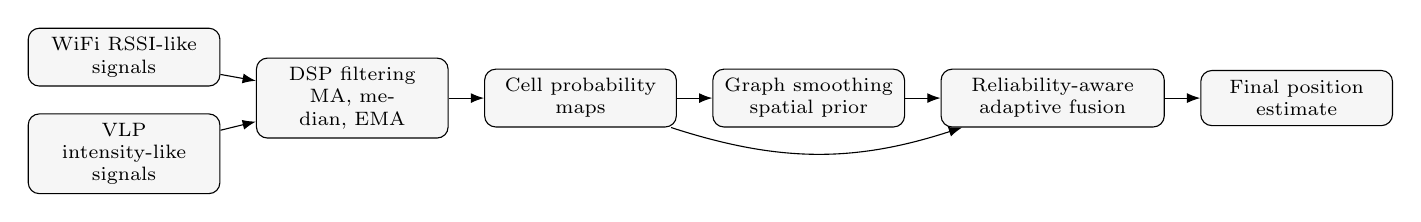
\begin{tikzpicture}[node distance=3.4mm and 4.5mm, >=Latex, every node/.style={font=\scriptsize}, box/.style={draw, rounded corners, align=center, minimum height=7mm, text width=22mm, fill=gray!7}]
\node[box] (wifi) {WiFi RSSI-like\\signals};
\node[box, below=of wifi] (vlp) {VLP intensity-like\\signals};
\node[box, right=of wifi, yshift=-5.2mm] (dsp) {DSP filtering\\MA, median, EMA};
\node[box, right=of dsp] (maps) {Cell probability\\maps};
\node[box, right=of maps] (gsp) {Graph smoothing\\spatial prior};
\node[box, right=of gsp, text width=26mm] (adapt) {Reliability-aware\\adaptive fusion};
\node[box, right=of adapt] (est) {Final position\\estimate};
\draw[->] (wifi) -- (dsp); \draw[->] (vlp) -- (dsp); \draw[->] (dsp) -- (maps); \draw[->] (maps) -- (gsp); \draw[->] (gsp) -- (adapt); \draw[->] (maps) to[bend right=18] (adapt); \draw[->] (adapt) -- (est);
\end{tikzpicture}
\caption{Processing pipeline. Graph smoothing supplies a spatial prior; the final policy combines it with modality maps according to reliability.}
\label{fig:pipeline}
\end{figure*}

For modality $m$, reliability is computed from peak probability and normalized entropy:
\begin{equation}
 q_m=\max(\mathbf{p}_{m})\left(1-\frac{H(\mathbf{p}_{m})}{\log 100}\right)\gamma_m,
 \label{eq:reliability}
\end{equation}
where $\gamma_m$ penalizes a known active degradation flag. The policy chooses among WiFi-heavy, VLP-heavy, balanced, graph-prior-heavy, and recovery modes. The final map is
\begin{equation}
 \mathbf{p}_{f}=\mathcal{N}\!\left(w_w\mathbf{p}_{w}+w_v\mathbf{p}_{v}+w_g\mathbf{p}_{g}\right).
 \label{eq:fusion}
\end{equation}
The weights are fixed per mode. Thus, the adaptive element is interpretable switching based on current reliability, not learned end-to-end localization.

\section{Experimental Setup}
We compare WiFi-only, VLP-only, equal-weight static fusion, static fusion after median DSP filtering, static fusion with graph diffusion, and the complete adaptive DSP+GSP fusion policy. Figures~\ref{fig:dsp} and \ref{fig:gsp} illustrate the two preprocessing components. The filters suppress short fluctuations but can lag or flatten useful clean measurements. Graph smoothing redistributes isolated peaks toward neighboring cells, which can stabilize a prior but can also blur a strong modality map. These tradeoffs motivate selective rather than unconditional use.

\begin{figure}[t]
\centering

\includegraphics[width=\columnwidth]{figures/fig3_noisy_vs_filtered_signals.png}
\caption{Representative noisy and DSP-filtered signal traces. Filtering reduces fluctuations but is not assumed to improve every localization case.}
\label{fig:dsp}
\end{figure}
\begin{figure}[t]
\centering

\includegraphics[width=\columnwidth]{figures/fig4_raw_vs_graph_smoothed_heatmap.png}
\caption{Example raw and graph-smoothed probability maps. The room graph spreads evidence locally across adjacent cells.}
\label{fig:gsp}
\end{figure}

\section{Results and Discussion}
\subsection{Scenario-wise results}
Table~\ref{tab:main} and Fig.~\ref{fig:error} show the main repeated-seed results. Static fusion is best in the clean scenario, with mean error $0.450\pm0.012$ m and P90 error $0.754\pm0.032$ m. VLP-only is best under WiFi degradation, with mean error $0.451\pm0.018$ m. In this controlled case, the optical modality remains clean, so a more elaborate fusion rule is unnecessary.

Adaptive fusion is most useful when the optical evidence is blocked or both modalities vary. Under VLP blockage, its mean error is $0.751\pm0.031$ m, compared with $1.013\pm0.092$ m for static fusion. Under mixed degradation, its mean error is $0.611\pm0.078$ m, compared with $0.759\pm0.101$ m for static fusion. Relative to static fusion, adaptive fusion improves mean error by 25.51\% and P90 error by 40.35\% in the VLP-blocked scenario. In the mixed-dynamic scenario, the corresponding improvements are 18.90\% and 26.20\%.

\begin{table*}[t]
\caption{Main Repeated-Seed Results (mean across five seeds; lower is better)}
\label{tab:main}
\centering
\scriptsize
\begin{tabular}{@{}llccc@{}}
\toprule
Scenario & Method & Mean (m) & P90 (m) & Fail. \\
\midrule
Clean & WiFi-only & 1.365 & 2.635 & .188 \\
 & VLP-only & .452 & .756 & .004 \\
 & Static fusion & \textbf{.450} & \textbf{.754} & \textbf{.004} \\
 & Adaptive fusion & .452 & .755 & .004 \\
\midrule
WiFi degraded & WiFi-only & 2.232 & 5.080 & .392 \\
 & VLP-only & \textbf{.451} & \textbf{.757} & .004 \\
 & Static fusion & .467 & .759 & .006 \\
 & Adaptive fusion & .451 & .757 & \textbf{.004} \\
\midrule
VLP blocked & WiFi-only & 1.369 & 2.792 & .192 \\
 & VLP-only & 1.015 & 2.689 & .170 \\
 & Static fusion & 1.013 & 2.667 & .168 \\
 & Adaptive fusion & \textbf{.751} & \textbf{1.578} & \textbf{.074} \\
\midrule
Mixed dynamic & WiFi-only & 1.918 & 3.986 & .336 \\
 & VLP-only & .759 & 1.749 & .100 \\
 & Static fusion & .759 & 1.749 & .100 \\
 & Adaptive fusion & \textbf{.611} & \textbf{1.198} & \textbf{.040} \\
\bottomrule
\end{tabular}

\end{table*}

\begin{figure}[t]
\centering

\includegraphics[width=\columnwidth]{figures/fig5_scenario_wise_error_paper.png}
\caption{Scenario-wise mean and P90 localization error across five seeds. Adaptive fusion is helpful under VLP blockage and mixed degradation, but it is not universally best.}
\label{fig:error}
\end{figure}

\subsection{DSP, GSP, failure rate, and smoothness}
Table~\ref{tab:ablation} isolates preprocessing effects in the two difficult scenarios. Median DSP reduces P90 error and failure rate under VLP blockage, and it gives the smoothest mixed-dynamic trajectories. Graph diffusion also reduces failure rate under VLP blockage. However, neither component alone dominates every metric: unconditional graph diffusion increases mixed-dynamic mean error. The complete adaptive policy benefits from choosing when to emphasize modality evidence and when to increase the graph-prior weight.

Fig.~\ref{fig:robust} shows the robustness summary. Against static fusion, adaptive fusion lowers failure rate by 0.094 under VLP blockage and by 0.060 under mixed degradation. Smoothness improves by 47.48\% and 40.50\%, respectively. These results support a conditional conclusion: adaptive weighting is useful when reliability changes, whereas clean or single-degradation settings may favor simpler estimators.

\begin{table}[t]
\caption{Ablation on Difficult Scenarios (lower is better)}
\label{tab:ablation}
\centering
\tiny
\begin{tabular}{@{}llcccc@{}}
\toprule
Scenario & Method & Mean & P90 & Fail. & Smooth. \\
\midrule
VLP blocked & Static fusion & 1.013 & 2.667 & .168 & 1.283 \\
 & + median DSP & .924 & 1.799 & .090 & .600 \\
 & + graph diffusion & .923 & 1.854 & .084 & 1.118 \\
 & Adaptive DSP+GSP & \textbf{.751} & \textbf{1.578} & \textbf{.074} & .672 \\
\midrule
Mixed dynamic & Static fusion & .759 & 1.749 & .100 & .917 \\
 & + median DSP & .794 & 1.362 & .044 & \textbf{.463} \\
 & + graph diffusion & 1.084 & 2.169 & .116 & 1.329 \\
 & Adaptive DSP+GSP & \textbf{.611} & \textbf{1.198} & \textbf{.040} & .535 \\
\bottomrule
\end{tabular}

\end{table}
\begin{figure}[t]
\centering

\includegraphics[width=\columnwidth]{figures/fig7_failure_smoothness_paper.png}
\caption{Failure rate and trajectory smoothness. The adaptive policy is most useful in the blocked and mixed-dynamic scenarios.}
\label{fig:robust}
\end{figure}

\section{Smartphone-Based Physical Sanity Check}
A small smartphone-based check was performed only to examine whether the simulation assumptions have the expected direction. The WiFi set contains 200 RSSI rows collected from 1--10 m under normal and blocked conditions. Mean normal RSSI changes from approximately $-29.1$ dBm at 1 m to $-49.1$ dBm at 10 m; the average blocked-minus-normal difference is $-14.95$ dB. The light set contains 200 app-estimated rows from 1--10 m under unblocked and blocked conditions. Mean unblocked intensity changes from approximately 627.7 to 39.1, and the average blocked/unblocked ratio is 0.0289. These trends motivate distance- and blockage-sensitive simulated degradation. The phone light-meter values are app estimates, not calibrated photodiode measurements, and this check is not a real localization implementation.

\section{Limitations}
This study is simulation-only. The RSSI-like model is simplified, the VLP intensity-like model is simplified, and neither is claimed as a new propagation model. The evaluation does not use WiFi channel state information, a camera receiver, a photodiode, or a deployed hybrid system. The adaptive policy is reliability-based rather than a new RL algorithm. Finally, the physical check is small and motivational; it is not full hardware or real-world localization validation. These boundaries limit generalization beyond the tested scenarios.

\section{Conclusion}
In the tested simulated setting, static fusion works best when both modalities are clean, VLP-only estimation works best when only WiFi is degraded, and reliability-aware adaptive fusion is most useful under optical blockage and mixed degradation. The adaptive policy reduces mean error relative to static fusion by approximately 25.51\% for VLP blockage and 18.90\% for mixed degradation while also reducing failures and improving smoothness. Future work should validate the approach with synchronized real WiFi and calibrated optical measurements, then study how the transparent policy behaves in deployed indoor environments.

\balance
\bibliographystyle{IEEEtran}
\bibliography{references}
\end{document}
